
%% bare_conf.tex
%% V1.3
%% 2007/01/11
%% by Michael Shell
%% See:
%% http://www.michaelshell.org/
%% for current contact information.
%%
%% This is a skeleton file demonstrating the use of IEEEtran.cls
%% (requires IEEEtran.cls version 1.7 or later) with an IEEE conference paper.
%%
%% Support sites:
%% http://www.michaelshell.org/tex/ieeetran/
%% http://www.ctan.org/tex-archive/macros/latex/contrib/IEEEtran/
%% and
%% http://www.ieee.org/

%%*************************************************************************
%% Legal Notice:
%% This code is offered as-is without any warranty either expressed or
%% implied; without even the implied warranty of MERCHANTABILITY or
%% FITNESS FOR A PARTICULAR PURPOSE!
%% User assumes all risk.
%% In no event shall IEEE or any contributor to this code be liable for
%% any damages or losses, including, but not limited to, incidental,
%% consequential, or any other damages, resulting from the use or misuse
%% of any information contained here.
%%
%% All comments are the opinions of their respective authors and are not
%% necessarily endorsed by the IEEE.
%%
%% This work is distributed under the LaTeX Project Public License (LPPL)
%% ( http://www.latex-project.org/ ) version 1.3, and may be freely used,
%% distributed and modified. A copy of the LPPL, version 1.3, is included
%% in the base LaTeX documentation of all distributions of LaTeX released
%% 2003/12/01 or later.
%% Retain all contribution notices and credits.
%% ** Modified files should be clearly indicated as such, including  **
%% ** renaming them and changing author support contact information. **
%%
%% File list of work: IEEEtran.cls, IEEEtran_HOWTO.pdf, bare_adv.tex,
%%                    bare_conf.tex, bare_jrnl.tex, bare_jrnl_compsoc.tex
%%*************************************************************************

% *** Authors should verify (and, if needed, correct) their LaTeX system  ***
% *** with the testflow diagnostic prior to trusting their LaTeX platform ***
% *** with production work. IEEE's font choices can trigger bugs that do  ***
% *** not appear when using other class files.                            ***
% The testflow support page is at:
% http://www.michaelshell.org/tex/testflow/



% Note that the a4paper option is mainly intended so that authors in
% countries using A4 can easily print to A4 and see how their papers will
% look in print - the typesetting of the document will not typically be
% affected with changes in paper size (but the bottom and side margins will).
% Use the testflow package mentioned above to verify correct handling of
% both paper sizes by the user's LaTeX system.
%
% Also note that the "draftcls" or "draftclsnofoot", not "draft", option
% should be used if it is desired that the figures are to be displayed in
% draft mode.
%
\documentclass[conference]{IEEEtran}
% Add the compsoc option for Computer Society conferences.
%
% If IEEEtran.cls has not been installed into the LaTeX system files,
% manually specify the path to it like:
% \documentclass[conference]{../sty/IEEEtran}


\makeatletter
\def\ps@headings{%
\def\@oddhead{\mbox{}\scriptsize\rightmark \hfil \thepage}%
\def\@evenhead{\scriptsize\thepage \hfil \leftmark\mbox{}}%
\def\@oddfoot{}%
\def\@evenfoot{}}
\makeatother

\pagestyle{headings}
\usepackage{amsfonts}
\usepackage{amsthm}
\usepackage{graphicx}
\usepackage{fancyhdr}
%\usepackage{floatflt}
%\usepackage{cite}
%\usepackage{balance}
%\usepackage{amssymb}
\usepackage{latexsym}


\newtheorem{Prop}{Proposition}
\newtheorem{lemma}{Lemma}
\newtheorem{theorem}{Theorem}


% Some very useful LaTeX packages include:
% (uncomment the ones you want to load)


% *** MISC UTILITY PACKAGES ***
%
%\usepackage{ifpdf}
% Heiko Oberdiek's ifpdf.sty is very useful if you need conditional
% compilation based on whether the output is pdf or dvi.
% usage:
% \ifpdf
%   % pdf code
% \else
%   % dvi code
% \fi
% The latest version of ifpdf.sty can be obtained from:
% http://www.ctan.org/tex-archive/macros/latex/contrib/oberdiek/
% Also, note that IEEEtran.cls V1.7 and later provides a builtin
% \ifCLASSINFOpdf conditional that works the same way.
% When switching from latex to pdflatex and vice-versa, the compiler may
% have to be run twice to clear warning/error messages.






% *** CITATION PACKAGES ***
%
%\usepackage{cite}
% cite.sty was written by Donald Arseneau
% V1.6 and later of IEEEtran pre-defines the format of the cite.sty package
% \cite{} output to follow that of IEEE. Loading the cite package will
% result in citation numbers being automatically sorted and properly
% "compressed/ranged". e.g., [1], [9], [2], [7], [5], [6] without using
% cite.sty will become [1], [2], [5]--[7], [9] using cite.sty. cite.sty's
% \cite will automatically add leading space, if needed. Use cite.sty's
% noadjust option (cite.sty V3.8 and later) if you want to turn this off.
% cite.sty is already installed on most LaTeX systems. Be sure and use
% version 4.0 (2003-05-27) and later if using hyperref.sty. cite.sty does
% not currently provide for hyperlinked citations.
% The latest version can be obtained at:
% http://www.ctan.org/tex-archive/macros/latex/contrib/cite/
% The documentation is contained in the cite.sty file itself.






% *** GRAPHICS RELATED PACKAGES ***
%
\ifCLASSINFOpdf
  % \usepackage[pdftex]{graphicx}
  % declare the path(s) where your graphic files are
  % \graphicspath{{../pdf/}{../jpeg/}}
  % and their extensions so you won't have to specify these with
  % every instance of \includegraphics
  % \DeclareGraphicsExtensions{.pdf,.jpeg,.png}
\else
  % or other class option (dvipsone, dvipdf, if not using dvips). graphicx
  % will default to the driver specified in the system graphics.cfg if no
  % driver is specified.
  % \usepackage[dvips]{graphicx}
  % declare the path(s) where your graphic files are
  % \graphicspath{{../eps/}}
  % and their extensions so you won't have to specify these with
  % every instance of \includegraphics
  % \DeclareGraphicsExtensions{.eps}
\fi
% graphicx was written by David Carlisle and Sebastian Rahtz. It is
% required if you want graphics, photos, etc. graphicx.sty is already
% installed on most LaTeX systems. The latest version and documentation can
% be obtained at:
% http://www.ctan.org/tex-archive/macros/latex/required/graphics/
% Another good source of documentation is "Using Imported Graphics in
% LaTeX2e" by Keith Reckdahl which can be found as epslatex.ps or
% epslatex.pdf at: http://www.ctan.org/tex-archive/info/
%
% latex, and pdflatex in dvi mode, support graphics in encapsulated
% postscript (.eps) format. pdflatex in pdf mode supports graphics
% in .pdf, .jpeg, .png and .mps (metapost) formats. Users should ensure
% that all non-photo figures use a vector format (.eps, .pdf, .mps) and
% not a bitmapped formats (.jpeg, .png). IEEE frowns on bitmapped formats
% which can result in "jaggedy"/blurry rendering of lines and letters as
% well as large increases in file sizes.
%
% You can find documentation about the pdfTeX application at:
% http://www.tug.org/applications/pdftex





% *** MATH PACKAGES ***
%
%\usepackage[cmex10]{amsmath}
% A popular package from the American Mathematical Society that provides
% many useful and powerful commands for dealing with mathematics. If using
% it, be sure to load this package with the cmex10 option to ensure that
% only type 1 fonts will utilized at all point sizes. Without this option,
% it is possible that some math symbols, particularly those within
% footnotes, will be rendered in bitmap form which will result in a
% document that can not be IEEE Xplore compliant!
%
% Also, note that the amsmath package sets \interdisplaylinepenalty to 10000
% thus preventing page breaks from occurring within multiline equations. Use:
%\interdisplaylinepenalty=2500
% after loading amsmath to restore such page breaks as IEEEtran.cls normally
% does. amsmath.sty is already installed on most LaTeX systems. The latest
% version and documentation can be obtained at:
% http://www.ctan.org/tex-archive/macros/latex/required/amslatex/math/





% *** SPECIALIZED LIST PACKAGES ***
%
%\usepackage{algorithmic}
% algorithmic.sty was written by Peter Williams and Rogerio Brito.
% This package provides an algorithmic environment fo describing algorithms.
% You can use the algorithmic environment in-text or within a figure
% environment to provide for a floating algorithm. Do NOT use the algorithm
% floating environment provided by algorithm.sty (by the same authors) or
% algorithm2e.sty (by Christophe Fiorio) as IEEE does not use dedicated
% algorithm float types and packages that provide these will not provide
% correct IEEE style captions. The latest version and documentation of
% algorithmic.sty can be obtained at:
% http://www.ctan.org/tex-archive/macros/latex/contrib/algorithms/
% There is also a support site at:
% http://algorithms.berlios.de/index.html
% Also of interest may be the (relatively newer and more customizable)
% algorithmicx.sty package by Szasz Janos:
% http://www.ctan.org/tex-archive/macros/latex/contrib/algorithmicx/




% *** ALIGNMENT PACKAGES ***
%
%\usepackage{array}
% Frank Mittelbach's and David Carlisle's array.sty patches and improves
% the standard LaTeX2e array and tabular environments to provide better
% appearance and additional user controls. As the default LaTeX2e table
% generation code is lacking to the point of almost being broken with
% respect to the quality of the end results, all users are strongly
% advised to use an enhanced (at the very least that provided by array.sty)
% set of table tools. array.sty is already installed on most systems. The
% latest version and documentation can be obtained at:
% http://www.ctan.org/tex-archive/macros/latex/required/tools/


%\usepackage{mdwmath}
%\usepackage{mdwtab}
% Also highly recommended is Mark Wooding's extremely powerful MDW tools,
% especially mdwmath.sty and mdwtab.sty which are used to format equations
% and tables, respectively. The MDWtools set is already installed on most
% LaTeX systems. The lastest version and documentation is available at:
% http://www.ctan.org/tex-archive/macros/latex/contrib/mdwtools/


% IEEEtran contains the IEEEeqnarray family of commands that can be used to
% generate multiline equations as well as matrices, tables, etc., of high
% quality.


%\usepackage{eqparbox}
% Also of notable interest is Scott Pakin's eqparbox package for creating
% (automatically sized) equal width boxes - aka "natural width parboxes".
% Available at:
% http://www.ctan.org/tex-archive/macros/latex/contrib/eqparbox/





% *** SUBFIGURE PACKAGES ***
%\usepackage[tight,footnotesize]{subfigure}
% subfigure.sty was written by Steven Douglas Cochran. This package makes it
% easy to put subfigures in your figures. e.g., "Figure 1a and 1b". For IEEE
% work, it is a good idea to load it with the tight package option to reduce
% the amount of white space around the subfigures. subfigure.sty is already
% installed on most LaTeX systems. The latest version and documentation can
% be obtained at:
% http://www.ctan.org/tex-archive/obsolete/macros/latex/contrib/subfigure/
% subfigure.sty has been superceeded by subfig.sty.



%\usepackage[caption=false]{caption}
%\usepackage[font=footnotesize]{subfig}
% subfig.sty, also written by Steven Douglas Cochran, is the modern
% replacement for subfigure.sty. However, subfig.sty requires and
% automatically loads Axel Sommerfeldt's caption.sty which will override
% IEEEtran.cls handling of captions and this will result in nonIEEE style
% figure/table captions. To prevent this problem, be sure and preload
% caption.sty with its "caption=false" package option. This is will preserve
% IEEEtran.cls handing of captions. Version 1.3 (2005/06/28) and later
% (recommended due to many improvements over 1.2) of subfig.sty supports
% the caption=false option directly:
%\usepackage[caption=false,font=footnotesize]{subfig}
%
% The latest version and documentation can be obtained at:
% http://www.ctan.org/tex-archive/macros/latex/contrib/subfig/
% The latest version and documentation of caption.sty can be obtained at:
% http://www.ctan.org/tex-archive/macros/latex/contrib/caption/




% *** FLOAT PACKAGES ***
%
%\usepackage{fixltx2e}
% fixltx2e, the successor to the earlier fix2col.sty, was written by
% Frank Mittelbach and David Carlisle. This package corrects a few problems
% in the LaTeX2e kernel, the most notable of which is that in current
% LaTeX2e releases, the ordering of single and double column floats is not
% guaranteed to be preserved. Thus, an unpatched LaTeX2e can allow a
% single column figure to be placed prior to an earlier double column
% figure. The latest version and documentation can be found at:
% http://www.ctan.org/tex-archive/macros/latex/base/



%\usepackage{stfloats}
% stfloats.sty was written by Sigitas Tolusis. This package gives LaTeX2e
% the ability to do double column floats at the bottom of the page as well
% as the top. (e.g., "\begin{figure*}[!b]" is not normally possible in
% LaTeX2e). It also provides a command:
%\fnbelowfloat
% to enable the placement of footnotes below bottom floats (the standard
% LaTeX2e kernel puts them above bottom floats). This is an invasive package
% which rewrites many portions of the LaTeX2e float routines. It may not work
% with other packages that modify the LaTeX2e float routines. The latest
% version and documentation can be obtained at:
% http://www.ctan.org/tex-archive/macros/latex/contrib/sttools/
% Documentation is contained in the stfloats.sty comments as well as in the
% presfull.pdf file. Do not use the stfloats baselinefloat ability as IEEE
% does not allow \baselineskip to stretch. Authors submitting work to the
% IEEE should note that IEEE rarely uses double column equations and
% that authors should try to avoid such use. Do not be tempted to use the
% cuted.sty or midfloat.sty packages (also by Sigitas Tolusis) as IEEE does
% not format its papers in such ways.





% *** PDF, URL AND HYPERLINK PACKAGES ***
%
%\usepackage{url}
% url.sty was written by Donald Arseneau. It provides better support for
% handling and breaking URLs. url.sty is already installed on most LaTeX
% systems. The latest version can be obtained at:
% http://www.ctan.org/tex-archive/macros/latex/contrib/misc/
% Read the url.sty source comments for usage information. Basically,
% \url{my_url_here}.





% *** Do not adjust lengths that control margins, column widths, etc. ***
% *** Do not use packages that alter fonts (such as pslatex).         ***
% There should be no need to do such things with IEEEtran.cls V1.6 and later.
% (Unless specifically asked to do so by the journal or conference you plan
% to submit to, of course. )


% correct bad hyphenation here
\hyphenation{op-tical net-works semi-conduc-tor}


\newcommand{\br}{{\mathbf r}}
\newcommand{\bA}{{\mathbf A}}
\newcommand{\ba}{{\bf a}}
\newcommand{\bb}{{\bf b}}
\newcommand{\bc}{{\bf c}}
\newcommand{\bC}{{\bf C}}
\newcommand{\bd}{{\bf d}}
\newcommand{\be}{{\bf e}}
\newcommand{\bE}{{\bf E}}
\newcommand{\bbf}{{\bf f}}
\newcommand{\bF}{{\bf F}}
\newcommand{\bh}{{\bf h}}
\newcommand{\bH}{{\bf H}}
\newcommand{\bg}{{\bf g}}
\newcommand{\bG}{{\bf G}}
\newcommand{\bq}{{\bf q}}
\newcommand{\bs}{{\bf s}}
\newcommand{\bm}{{\bf m}}
\newcommand{\bn}{{\bf n}}
\newcommand{\bu}{{\bf u}}
\newcommand{\bv}{{\bf v}}
\newcommand{\bw}{{\bf w}}
\newcommand{\bx}{{\bf x}}
\newcommand{\by}{{\bf y}}
\newcommand{\bz}{{\bf z}}
\newcommand{\bL}{{\bf L}}
\newcommand{\bM}{{\bf M}}
\newcommand{\bN}{{\bf N}}
\newcommand{\bS}{{\bf S}}
\newcommand{\bT}{{\bf T}}
\newcommand{\bD}{{\bf D}}
\newcommand{\bX}{{\bf X}}
\newcommand{\bP}{{\bf P}}
\newcommand{\bQ}{{\bf Q}}
\newcommand{\bI}{{\bf I}}
\newcommand{\bR}{{\bf R}}
\newcommand{\bU}{{\bf U}}
\newcommand{\bV}{{\bf V}}
\newcommand{\bW}{{\bf W}}
\newcommand{\bY}{{\bf Y}}
\newcommand{\bZ}{{\bf Z}}
\newcommand{\bJ}{{\bf J}}
\newcommand{\bB}{{\bf B}}
\newcommand{\bzero}{{\bf 0}}
\newcommand{\bgamma}{{\mbox {\boldmath $\gamma$}}}
\newcommand{\btheta}{{\mbox {\boldmath $\theta$}}}
\newcommand{\bvartheta}{{\mbox {\boldmath $\vartheta$}}}
\newcommand{\bDelta}{{\mbox {\boldmath $\Delta$}}}
\newcommand{\bLambda}{{\mbox {\boldmath $\Lambda$}}}
\newcommand{\bPsi}{{\mbox {\boldmath $\Psi$}}}
\newcommand{\bPhi}{{\mbox {\boldmath $\Phi$}}}
\newcommand{\bcA}{{\mbox {\boldmath ${\cal A}$}}}
\newcommand{\bcB}{{\mbox {\boldmath ${\cal B}$}}}
\newcommand{\bcC}{{\mbox {\boldmath ${\cal C}$}}}
\newcommand{\bcD}{{\mbox {\boldmath ${\cal D}$}}}
\newcommand{\bcF}{{\mbox {\boldmath ${\cal F}$}}}
\newcommand{\bcG}{{\mbox {\boldmath ${\cal G}$}}}
\newcommand{\bcL}{{\mbox {\boldmath ${\cal L}$}}}
\newcommand{\bcN}{{\mbox {\boldmath ${\cal N}$}}}
\newcommand{\bcR}{{\mbox {\boldmath ${\cal R}$}}}
\newcommand{\bcS}{{\mbox {\boldmath ${\cal S}$}}}
\newcommand{\bcH}{{\mbox {\boldmath ${\cal H}$}}}
\newcommand{\bcI}{{\mbox {\boldmath ${\cal I}$}}}
\newcommand{\bcO}{{\mbox {\boldmath ${\cal O}$}}}
\newcommand{\bcP}{{\mbox {\boldmath ${\cal P}$}}}
\newcommand{\bcQ}{{\mbox {\boldmath ${\cal Q}$}}}
\newcommand{\bcV}{{\mbox {\boldmath ${\cal V}$}}}
\newcommand{\bcW}{{\mbox {\boldmath ${\cal W}$}}}


\begin{document}
%
% paper title
% can use linebreaks \\ within to get better formatting as desired
\title{On Enhancing Hierarchical Modulation}


% author names and affiliations
% use a multiple column layout for up to three different
% affiliations
\author{\IEEEauthorblockN{Shu Wang, Byung K. Yi and Soonyil Kwon}
%\author{\IEEEauthorblockN{Diet Koffee}
\IEEEauthorblockA{LG Electronics Mobile Research\\
San Diego, CA 92131-1639\\
Email: \{swang,\ byungkyi,\ sykown\}@lge.com} }
%Email: dietkoffee@lge.com} }

% conference papers do not typically use \thanks and this command
% is locked out in conference mode. If really needed, such as for
% the acknowledgment of grants, issue a \IEEEoverridecommandlockouts
% after \documentclass

% for over three affiliations, or if they all won't fit within the width
% of the page, use this alternative format:
%
%\author{\IEEEauthorblockN{Michael Shell\IEEEauthorrefmark{1},
%Homer Simpson\IEEEauthorrefmark{2},
%James Kirk\IEEEauthorrefmark{3},
%Montgomery Scott\IEEEauthorrefmark{3} and
%Eldon Tyrell\IEEEauthorrefmark{4}}
%\IEEEauthorblockA{\IEEEauthorrefmark{1}School of Electrical and Computer Engineering\\
%Georgia Institute of Technology,
%Atlanta, Georgia 30332--0250\\ Email: see http://www.michaelshell.org/contact.html}
%\IEEEauthorblockA{\IEEEauthorrefmark{2}Twentieth Century Fox, Springfield, USA\\
%Email: homer@thesimpsons.com}
%\IEEEauthorblockA{\IEEEauthorrefmark{3}Starfleet Academy, San Francisco, California 96678-2391\\
%Telephone: (800) 555--1212, Fax: (888) 555--1212}
%\IEEEauthorblockA{\IEEEauthorrefmark{4}Tyrell Inc., 123 Replicant Street, Los Angeles, California 90210--4321}}

% use for special paper notices
%\IEEEspecialpapernotice{(Invited Paper)}

% make the title area

\maketitle
\begin{abstract}\small
Interference cancellation is one of the major multiuser detection
strategies for suppressing interference effects and improving
system performance. In this paper, a novel blind decision-feedback
interference cancellation framework and several implementations
with least squares, maximum likelihood and minimum mean squared
error criteria are proposed for solving the CDMA near-far problem.
Compared with existing blind multiuser receivers, the proposed
approaches require a minimum number of previous received signals
with no subspace separation or sequence estimation. Therefore the
detection complexity and delay can be lower, especially when this
framework can be adaptively and/or iteratively implemented for
further improving detection performance. Theoretical analysis and
comparison with existing multiuser receivers as well as computer
simulations are provided to demonstrate the performance of the
proposed schemes.
\end{abstract}
\section{Introduction}
Interference cancellation (IC) is the strategy for forming an
estimate of incurred interference, like intersymbol interference
(ISI), co-channel interference (CCI), adjacent channel
interference (ACI), etc., and subtracting it from received signals
before detection. Compared with other detection strategies,
interference cancellation strategy focuses more on interference
estimation. And different interference estimation methods may lead
to different interference cancellation
schemes~\cite{Verd98,Wang02b}, e.g. successive cancellation,
multistage detection, decision-feedback interference cancellation
(DFIC)~\cite{Kave85,Duel95}, etc. DFIC, including minimum mean
squared error (MMSE) DFIC~\cite{Kave85} and decorrelating
DFIC~\cite{Duel95}, is the decision-driven detection scheme that
combines features of successive interference cancellation and
multistage detection~\cite{Verd98}. Conventional multiuser
receivers including conventional interference cancellation are
known to be able to solve the near-far problem with the knowledge
of the signature information of all users~\cite{Verd98}. However
this assumption isn't consistent with many practical situations
where the receiver may only know the signatures of the expected
signals not interfering signals. Recent research has been devoted
to semiblind/blind implementation of interference cancellation as
well as other multiuser
detectors~\cite{Madh94,Wang98,Zhang02,Wang03d,Wang05A} for the
practical applications where only information of desired/known
user(s) is available. In existing semiblind/blind implementations,
adaptive filter techniques, e.g., Wiener filtering~\cite{Madh94},
Kalman filtering~\cite{Zhang02} and subspace-based
implementations~\cite{Wang98}, are among the most popular choices.

Decision-feedback techniques, including decision-feedback channel
equalization and signal detection, have intensively been discussed
since 1960s. In single-user decision-feedback equalization (DFE),
previous decision outputs are feeded back for estimating ISI and
detecting the next symbol. DFE is known to have the complexity
close to linear equalization while the performance is close to
maximum likelihood equalization. In multiuser DFIC, both current
and previous received symbols and decision outputs are utilized
for detecting desired user(s)'s data~\cite{Verd98}. In
conventional DFIC~\cite{Verd98}, other users' current decision
outputs as well as their signal signatures are usually used for
estimating interference and detecting desired information. In
blind DFIC, only received signals and detection outputs of the
desired user(s) are available for separating signal subspaces
and/or adapting receiver for better interference
estimation~\cite{Wang98}. The challenge with most existing DFIC
receiver design is that neither subspace separation nor receiver
adapting procedure is simple and fast enough for fast-fading
channels~\cite{Madh94,Wang98,Zhang02}. In some situations, there
even is no enough received coherent signals for training the blind
multiuser receivers.

Conventional multiuser receivers as well as the blind interference
cancellation receiver with a large number of previously received
symbols have been intensively investigated so far. However, the
performance of blind interference cancellation receiver with
limited previous knowledge is largely unknown. In order to solve
the near-far problem with minimum prior knowledge as well as
computation complexity and delay~\cite{Wang03d,Wang05A}, we
provide an alternative blind DFIC multiuser receiver design
framework, in which only a small amount of previous received
symbols are required for estimating interference and detecting
next symbols in addition to desired user(s)' signatures and
timing. The trick is, instead of using previous received symbols
for signal signature estimation or signal subspace separation,
they are directly taken as signal space bases, termed {\em blind
signal signatures}, for separating interference from received
signals. Thereafter, with different signal estimation criteria,
including least squares (LS), maximum likelihood (ML) and MMSE,
several blind interference cancellation receivers are constructed.
It is also shown that the proposed framework can be implemented in
adaptive and/or iterative fashion so that the incurred complexity
and detection delay can be further reduced. All these make it an
attractive candidate to design blind interference cancellation
receiver for high data rate systems. Theoretical analysis and
comparison and computer simulations are finally presented to
demonstrate the performance of these blind detectors. The proposed
framework and approaches can easily be extended for asynchronous
CDMA too.
\section{System Model And Problem Description}
The synchronous transmissions in a single-cell DS/CDMA system with
$K$ active users is discussed here. The channel is a multiplath
channel with $P$ strong paths~\footnote{Strong paths are those to
be explicitly combined by RAKE receiver.} and corrupted by
additive white Gaussian noise (AWGN). The baseband representation
of the received signal due to user $k$ is given by
\begin{equation}
\begin{array}{l}\hspace{-0.2in}
r_k(t)=\sum\limits_{p=1}^{P}\alpha_{pk}A_k[n]
b_k[n]c_k(t-nT-\tau_p)+n_k(t)
\end{array}
\end{equation}
\noindent where $\alpha_{pk}$ is the $p$th path loss of user $k$'s
signal, $b_k{[n]}$ is the $n$th bit sent by user $k$. We assume
that the $\left\{b_k{[n]}\right\}$ are independent and identically
distributed random variables with $E\left\{b_k{[i]}\right\}=0$ and
$E\left\{|b_k{[i]}|^2\right\}=1$. The parameters $c_k(t)$ denote
the normalized spreading signal waveform of user $k$ during the
interval $[0,\ T]$, $0\leq\tau_1\leq\tau_2\leq\ldots\leq\tau_P$,
denotes $P$ different transmission delays from the base station to
user $k$ and $A_k[n]$ is the received signal amplitude for user
$k$ at time $t=nT$, which depends on the possible channel
statistics. The total baseband signal received by user $k$ is
\begin{equation}
\begin{array}{rcl}
\tilde{r}(t)&=&\sum\limits_{k=1}^{K}r_k(t)
\end{array}
\end{equation}
The received signal $\tilde{r}(t)$ is passed through the
corresponding chip matched filter (CMF), $\phi(t)$, and RAKE
combiner. The combined output $r(t)$ is~\footnote{We drop the time
index $n$ in the following discussion when it refers to the
current signal.}
\begin{equation}\hspace{-0.0in}
\begin{array}{rcl}
r(t)&=&A_k b_k c_k(t-nT-\tau_1)\otimes \phi(t-\tau_1)+ \\
&&\hspace{0.0in} m_{\rm ISI}(t) + m_{\rm MAI}(t) + n(t)
\end{array}\label{r_t}
\end{equation}
\noindent where
\begin{equation} \hspace{-0.05in}
\begin{array}{rcl}
 m_{\rm ISI}(t)&=&\\
 &&\hspace{-0.83in}\sum\limits^{p,q=P}_{p\neq
q}\beta_{qk} \alpha_{pk}A_kb_kc_k(t-nT+\tau_{q1}-\tau_1)\otimes
\phi(t-\tau_1)
\end{array}
\end{equation}
\noindent is the intersymbol interference (ISI) to user $k$,
\begin{equation} \hspace{-0.07in}
\begin{array}{l}
m_{\rm MAI}(t)=\sum\limits_{i\neq
 k}^{K}A_ib_ic_i(t-nT-\tau_1)\otimes\phi(t-\tau_1)+\\
 \hspace{-0.05in}\sum\limits_{i\neq
 k}^{K}\sum\limits^{p,q=P}_{p\neq
q}\beta_{qk}
\alpha_{pi}A_ib_ic_i(t-nT+\tau_{q1}-\tau_p)\otimes\phi(t-\tau_1)
\end{array}
\end{equation}
\noindent is the MAI to user $k$, $\beta_{qk}$ is the weight of
the $q$th RAKE finger with
\begin{equation}
\begin{array}{rcl}
\sum\limits_{q=1}^{P}\beta_{qk}\alpha_{qk}&=&1
\end{array}
\end{equation}
\noindent and $\tau_{q1} = \tau_{q}-\tau_1$ is the propagation
delay difference between the $1$st path and $p$th path. $\otimes$
denotes the convolutional product. $n(t)$ is AWGN with variance
$\sigma^2$. Furthermore, the user $k$'s RAKE output can be sampled
at $f_s=\frac{1}{T_s}$ and straightforwardly expressed
by~\cite{Verd98}
\begin{equation}\hspace{-0.18in}
\begin{array}{l}
\br=\left[
\matrix{r(nT+T_s+\tau_1)&\ldots&r(nT+LT_s+\tau_1)}\right]^{\rm
T}\\
\hspace{0.1in}=\sum\limits_{k=1}^{K} A_k b_k \bs_k + \bn \\
\hspace{0.1in}=\bS \bA \bb + \bn
\end{array}\label{r_sync}
\end{equation}
\noindent where $\bS=\left[\bs_1\ \bs_2\ \ldots\ \bs_K\right]$ is
the received spreading sequence matrix combined with both ISI and
MAI information, and $L=\frac{T}{T_s}$ is the number of samples
per symbol, which usually is not less than the spreading gain
$L_c$. Because of $m_{\rm MAI}(t)$ existing in the received signal
$r(t)$, the performance of conventional matched filter receiver
suffers from the so-called near-far problem and interference
cancellation is one of the receiver techniques for solving this
problem~\cite{Verd98}. However, most existing interference
cancellation receivers are designed with the assumption that
either the knowledge of the signature information of all user or a
large number of previous received signals is available. This
assumption isn't consistent with many practical situations where
the receiver may only know the signatures of the expected signals
not interfering signals. In following sections, a blind
interference cancellation framework and several implementation of
it are presented with only several previous received signals.
\section{Blind Decision-Feedback Interference Cancellation Framework}
Without loss of the generality, the signals for the first $G$
desired users will be detected with the assumption
$\bS_1=\left[\matrix{\bs_1&\bs_2&\ldots&\bs_G}\right]$ is known
beforehand. With (\ref{r_sync}) and $\bb=\left[\bb_{1}^{\rm H}\
\bb_{2}^{\rm H}\right]^{\rm T}$, $\bb_{1}=\left[b_{1}\ \cdots\
b_{G}\right]^{\rm H}$ is the data vector we want to detect and
$\bb_{2}=\left[b_{G+1}\ \cdots\ b_{K}\right]^{\rm T}$ is the data
vector embedded in interference. For the estimation of the MAI to
the first $G$ users, we assemble $M$ previously received and
detected signal vectors into
\begin{equation}
\begin{array}{rcl}
\bcS&=&\bigl[\matrix{{\br}[n-1]&{\br}[n-2]&\ldots&{\br}[n-M]}\bigr]\\
&=&\bS\bA\bB+\bN\\
&=&\bS_1\bA_1\bB_1+\bS_2\bA_2\bB_2+\bN
\end{array} \label{bcs}
\end{equation}
\noindent where $\left\{\br[n-m]:\ 1\leq m\leq M\right\}$ denotes
previously received and detected $M$ signals,
\begin{equation}
\begin{array}{rcl}
\bB=\left[\matrix{\bB_1\cr\bB_2}\right]
\end{array}
\end{equation}
\noindent is the data matrix for $\bcS$, $\bS_2$ is the original
interfering signals' signatures, $\bA_1$, $\bA_2$, $\bB_1$ and
$\bB_2$ are the amplitude matrices and data matrices for desired
users and interfering users, respectively, and $\bN$ is a AWGN
matrix. Obviously the minimum number of received signals a
receiver requires for clearly identifying the $\left(K-G\right)$
interfering users is $M=K-G$ with ${\rm
rank}\left(\bB_2\right)=K-G$. With (\ref{bcs}), the interference
subspace can be approximated by
$\bar\mathbb{S}_{1}=\mbox{span}\left\{\bs_m | m=G+1,\ \ldots\
K\right\}\approx\mbox{span}\left\{\bcS-\bS_1\bA_1\bB_1\right\}$.
And the MAI $\bm$ can be rewritten by
\begin{equation}\hspace{-0.0in}
\begin{array}{rcl}
\bm &=&\bS_2\bA_2\bb_2\\
&=&\bigl(\bcS-\bS_1\bA_1\bB_1-\bN\bigr)\bB_2^{+}\bb_2\\
&=&\bcS\bbf-\bS_1\bD_1\bbf+\tilde{\bn}
\end{array}\label{bm}
\end{equation}
\noindent where $\bbf=\bB_2^{+}\bb_2$ denotes a projection of
$\bm$ onto the interfering subspace of $\bS_2\bA_2\bB_2$,
$\bD_1=\bA_1\bB_1$ and $\tilde{\bn}=-\bN\bB_2^{+}\bb_2$.
$[\cdot]^{+}$ denotes the general inverse.

With (\ref{bm}), it shows that $\bm$ can be estimated providing
$\bbf$ is known. In order to estimate $\bbf$, we perform
QR-decomposition on $\bS_1$ so that~\cite{Huff91,Verd98}
\begin{equation}
\begin{array}{rcccl}
\bS_1&=&\bQ_1\bR_1&=&\bQ_{11}\bR_{11}
\end{array},
\end{equation}
\noindent where $\bQ_1=\left[\bQ_{11}\
\bQ_{12}\right]\in\mathbb{R}^{L\times L}$ is orthogonal and
$\bR_1=[\bR_{11}^{\rm H}\ \bzero^{\rm H}]^{\rm
H}\in\mathbb{R}^{L\times G}$, and apply $\bQ_{12}^{\rm H}$ on
(\ref{bm}) to get
\begin{equation}
\begin{array}{rcl}
\bQ_{12}^{\rm H}\bm&=&\bQ_{12}^{\rm H}\bcS\bbf+\bQ_{12}^{\rm
H}\tilde\bn
\end{array}.
\end{equation}
\noindent Since
\begin{equation}\hspace{-0.0in}
\begin{array}{rcl}
\bQ_{12}^{\rm H}\br&=&\bQ_{12}^{\rm H}\bm + \bQ_{12}^{\rm H}\bn
\end{array},
\end{equation}
\noindent $\bbf$ can be estimated from
\begin{equation}\hspace{-0.0in}
\begin{array}{rcl}
\bQ_{12}^{\rm H}\br&=&\bQ_{12}^{\rm H}\bcS\bbf+\bQ_{12}^{\rm
H}\bar\bn
\end{array},\label{f2}
\end{equation}
\noindent where $\bar\bn=\tilde\bn+\bn$.

After $\bbf$ is estimated, $\bm$ can be estimated using (\ref{bm})
and extracted from $\br$ so that the desired information vector
$\bb_1$ as well as $\bA_1$ can be detected and estimated from
\begin{equation}
\begin{array}{rcl}
\bS_1\bd_1&\approx&\br-\left(\bcS-\bS_1\hat\bD_1\right)\hat{\bbf}
\end{array},\label{br_bm}
\end{equation}
\noindent where $\bd_1=\bA_1\bb_1$, $\hat\bD_1$ denotes previous
detection outputs from $\bcS$ and $\hat{\bbf}$ denotes an estimate
of $\bbf$. This can be done using either Viterbi algorithm or
other sub-optimal detection schemes. This can be shown in Fig. 1.
Since the previous decision outputs $\hat\bD_1$ are used for
estimating $\bm$ and $\bA_1$ and detecting $\bb_1$, this framework
is named blind decision-feedback interference cancellation. Though
this framework is presented as a two-stage approach here, it can
be implemented in a joint detection fashion with simultaneously
estimating $\bd_1$ and $\bbf$.
\begin{figure} \center{
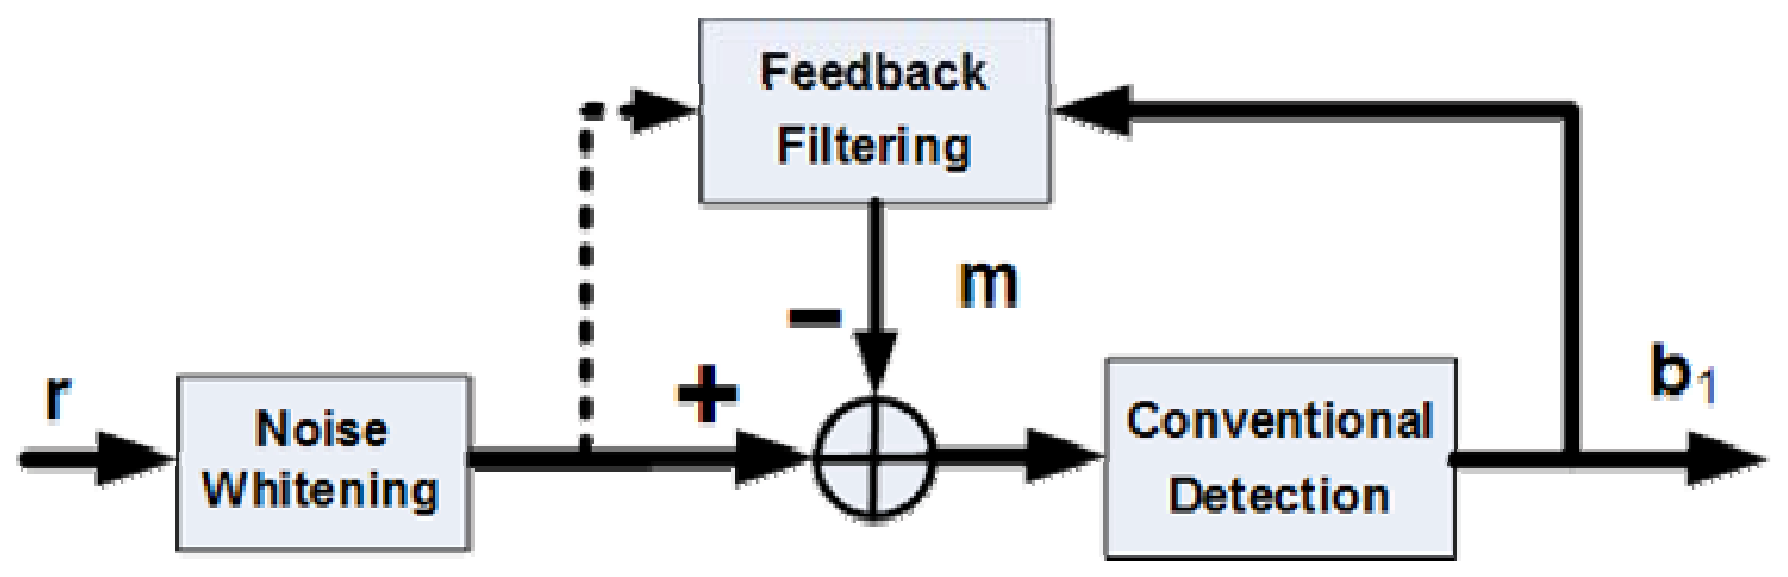
\includegraphics[width=3.2in]{BDFIC1.eps}
\caption{A decision feedback interference cancellation block
diagram} }\label{DFIC}
\end{figure}
\section{Blind Decision-Feedback Interference Cancellation Implementations}
\subsection{\em Least Squares Interference Cancellation}
In traditional least squares estimations, the observation matrix
is assumed to be error-free and all estimation errors are supposed
to come from $\br$. This can be formulated by
\begin{equation}\hspace{-0.09in}
\begin{array}{rcl}
\left[\matrix{{\bd}_{1\rm LS}\cr\bbf_{\rm
LS}}\right]&=&\mbox{arg}\min\limits_{\bx}\left\|\br-\bG\bx\right\|_2
\end{array}\label{prob_LS}
\end{equation}
\noindent where
\begin{equation}
\begin{array}{rcl}
\bG&=&\left[\matrix{\bS_1&\left(\bcS-\bS_1\bD_1\right)}\right]
\end{array}.
\end{equation}
\noindent Now $\bd_1$ as well as $\bbf$ can therefore be estimated
by
\begin{equation}\hspace{-0.0in}
\begin{array}{rcl}
\left[\matrix{{\bd}_{1\rm LS}\cr\bbf_{\rm
LS}}\right]&=&\bG^{+}\br.
\end{array}\label{b_LS_IC}
\end{equation}

Besides the traditional LS assumption, another one is to assume
both $\bG$ and $\br$ are noise-polluted so that (\ref{prob_LS})
becomes the total least squares (TLS) problem
\begin{equation}\hspace{-0.12in}
\begin{array}{rcl}
\left[\matrix{{\bG}_{\rm TLS}\cr\left[\matrix{{\bd}_{1\rm
TLS}\cr\bbf_{\rm
TLS}}\right]}\right]&=&\mbox{arg}\min\limits_{\bY,\
\bx}\left\|\left[\matrix{\bG\cr\br}\right]-\left[\matrix{\bY\cr\bY\bx}\right]\right\|_2
\end{array}.\label{prob_TLS}
\end{equation}
Let $\bG=\bU^{'}\mathbf{\Sigma}^{'}\bV^{'\rm T}$ and $[\bG\
\br]=\bU\mathbf{\Sigma}\bV^{\rm T}$ be the SVD of $\bG$ and $[\bG\
\br]$, respectively. If $\sigma_K^{'}
> \sigma_{K+1}$, the TLS estimation of $\bd_{1}$ and $\bbf$ is
\begin{equation}
\begin{array}{rcl}
\left[\matrix{{\bd}_{1\rm TLS}\cr\bbf_{\rm
TLS}}\right]&=&\left(\bG^{\rm
T}\bG-\sigma_{K+1}^2\bI\right)^{-1}\bG^{\rm T}\br
\end{array}
\end{equation}

It seems that either (\ref{prob_LS}) or (\ref{prob_TLS}) is not
accurate since $\bS_1$ is known to be noise-free and $\bcS$ is
noise-corrupted. It seems that it is more reasonable to require
$\bS_1$ to be unperturbed while keep $\bcS$ estimated. Therefore
it leads to a mixed least squares (MLS) interference cancellation
problem expressed by
\begin{equation}\hspace{-0.07in}
\begin{array}{l}
\left[\matrix{{\bcS}_{\rm
MLS}\cr\left[\matrix{{\bd}_{1}+\bD_{1}\bbf\cr\bbf}\right]_{\rm
MLS}}\right]=\mbox{arg}\min\limits_{\bZ,\
\by}\left\|\left[\matrix{\bcS\cr\br}\right]-\left[\matrix{\bZ\cr\left[\bS_1\
\bZ\right]\by}\right]\right\|_2
\end{array}.
\end{equation}
\noindent If $\sigma_{K-G}'>\sigma_{K-G+1}$, the MLS estimation of
$\bbf$ is
\begin{equation}\hspace{-0.070in}
\begin{array}{l}
{\bbf_{\rm MLS}}=\left(\bcS^{\rm H}\bQ_{12}\bQ_{12}^{\rm
H}\bcS-\sigma_{K-G+1}^{2}\bI\right)^{-1}\bcS^{\rm
H}\bQ_{12}\bQ_{12}^{\rm H}\br
\end{array}\label{f_MLS}
\end{equation}
\noindent where $\sigma_{K-G}'$ and $\sigma_{K-G+1}$ are the
$(K-G)$th and $(K-G+1)$th largest singular value of $\bQ_{12}^{\rm
H}\bcS$ and $\bQ_{12}^{\rm H}\left[\matrix{\br&\bcS}\right]$. The
MLS-IC ${\bd}_{1\rm MLS}$ can be expressed by
\begin{equation}\hspace{0.0in}
\begin{array}{rcl}
{\bd}_{1\rm
MLS}&=&\bS_{1}^{+}\br-\bS_{1}^{+}\left({\bcS}-{\bS}_{1}{\bD_1}\right){\bbf_{\rm
MLS}}
\end{array}\label{b_MLS_IC}
\end{equation}
\subsection{\em Maximum Likelihood Interference Cancellation}
In maximum likelihood interference cancellation (ML-IC), $\bd_1$
is estimated with maximizing the probability density function
(PDF) $p(\br;\ \bd_{1},\ \bbf)$. It is known that ML estimator
asymptotically is the minimum variance unbiased (MVU) estimator
though it is not optimal in general. For the linear Gaussian
signal model in (\ref{br_bm}), ML-IC can be written by
\begin{equation}\hspace{-0.12in}
\begin{array}{rcl}
\left[\matrix{{\bd}_{1\rm ML}\cr\bbf_{\rm
ML}}\right]&=&\mbox{arg}\min\limits_{\bx}\left\{\mathbf\delta^{\rm
H}\bR_{\bar\bn}\mathbf\delta\right\}
\end{array}
\end{equation}
\noindent where the estimation error vector
\begin{equation}
\begin{array}{rcl}
\mathbf\delta&=&\br-\bG\bx
\end{array}.
\end{equation}
Therefore the ML estimation of $\bd_1$ can be given by
\begin{equation}
\begin{array}{rcl}
\left[\matrix{{\bd}_{1\rm ML}\cr\bbf_{\rm
ML}}\right]&=&\left(\bG^{\rm
H}\bR_{\bar\bn}\bG\right)^{-1}\bG^{\rm H}\bR_{\bar\bn}^{-1}\br
\end{array}.\label{b_ML_IC}
\end{equation}
\subsection{\em Mini. Mean-Square Error Interference Cancellation}
With MMSE criterion, $\bd_{1}$ is estimated with minimizing the
Bayesian mean squared error (BMSE):
\begin{equation}\hspace{-0.0in}
\begin{array}{rcl}
\be_{\rm
BMSE}&=&\mbox{E}\left\|\left[\matrix{\hat\bd_{1}\cr\hat\bbf}\right]-\left[\matrix{\bd_{1}\cr\bbf}\right]\right\|_2^2
\end{array}.
\end{equation}
\noindent The MMSE estimation can then be written by
\begin{equation}\hspace{-0.15in}
\begin{array}{l}
\left[\matrix{{\bd}_{1\rm MMSE}\cr\bbf_{\rm
MMSE}}\right]=\mbox{arg}\min\limits_{\bx}\mbox{E}\left\|\br-\bG\bx\right\|_2
\end{array}\label{MMSE_IC}
\end{equation}
\noindent and, if $\br$, $\bd_{1}$ and $\bbf$ are jointly
Gaussian, it can be solved by
\begin{equation}\hspace{-0.15in}
\begin{array}{rcl}
\left[\matrix{{\bd}_{1\rm MMSE}\cr\bbf_{\rm
MMSE}}\right]&=&\left(\bR_{\bx}+\bG^{\rm
H}\bR_{\bar\bn}\bG\right)^{-1}\bG^{\rm H}\bR_{\bar\bn}^{-1}\br
\end{array}\label{b_MMSE_IC}
\end{equation}
\noindent where
\begin{equation}
\begin{array}{rcl}
\bR_{\bx}&=&\mbox{E}\left\{\left[\matrix{\bd_{1}\bd_{1}^{\rm
H}&\bd_{1}\bbf^{\rm H} \cr \bbf\bd_{1}^{\rm H}&\bbf\bbf^{\rm
H}}\right]\right\}
\end{array}.%\label{b_ML_IC}
\end{equation}
\section{Implementation Considerations}
\subsection{\em Adaptive Detection}
When transmitted signals experience channel condition changes, it
is better for the receiver to response fast enough to follow this
change with minimum adaptive lag. With (\ref{bcs}) and
(\ref{br_bm}), it shows that the proposed DFIC framework $M$
previously received symbols for the next detection so that it may
be able to track channel fast. Since its implementations typically
involve the inverse of $\bG^{\rm H}\bG$ in (\ref{b_LS_IC}),
$\bG^{\rm H}\bR_{\bar\bn}\bG$ in (\ref{b_ML_IC}), etc., one of the
possible approaches is to follow the well-known
Sherman-Morrison-Woodbury matrix inverse lemma~\cite{Haykin96}.
For example, if we define
\begin{equation}
\begin{array}{rcl}
\bPhi[n]&=&\bG^{\rm H}[n]\bG[n]
\end{array},\label{R_G}
\end{equation}
\noindent where $\bG[n]$ denotes the instance of $\bG$ at $t=n$,
so that $\bPhi[n+1]$ can be rewritten by
\begin{equation}
\begin{array}{rcl}
\bPhi[n+1]&=&\bPhi[n] + \bu[n]\bu^{\rm H}[n]
\end{array}.
\end{equation}
The inverse of $\bPhi[n+1]$ can be recursively calculated by
\begin{equation}\hspace{-0.08in}
\begin{array}{l}
\bPhi^{-1}[n+1]=\bPhi^{-1}[n]-\frac{\bPhi^{-1}[n]\bu[n]\bu^{\rm
H}[n]\bPhi^{-1}[n]}{1+\bu^{\rm H}[n]\bPhi^{-1}[n]\bu[n]}
\end{array}.\label{adaptiveLS}
\end{equation}
\subsection{\em Iterative Detection}
The presented detection framework can be generalized by solving
the following optimization problem:
\begin{equation}
\begin{array}{rcl}
\hat{\bd}_{1}&=&\min{f\left(\br;\ \bcS,\hat{\bD}_1\right)}
\end{array},\label{generalFramework}
\end{equation}
\noindent which subject to some possible constraints, where the
$f\left(\cdot\right)$ is the objective function. Iterative
detection is one the approaches for solving this optimization
problem. For this, (\ref{generalFramework}) may be extended to
\begin{equation}
\begin{array}{rcl}
\hat{\bd}_{1}&=&\min{f\left(\br;\ \left[\bcS\
\br\right],\left[\hat{\bD}_1\ \hat{\bd}_1\right]\right)}
\end{array}.\label{extendedFramework}
\end{equation}
And one iterative framework for solving (\ref{extendedFramework})
can be expressed by
\begin{equation}\hspace{-0.05in}
\begin{array}{rcl}
\hat{\bd}_{1}[n+1]&=&\min{f\left(\br;\ \left[\bcS\
\br\right],\left[\hat{\bD}_1\ \hat{\bd}_1[n]\right]\right)}
\end{array}.
\end{equation}
\subsection{\em Coded Blind Interference Cancellation}
In reality, an IC detector will cancel the interfering signal
exactly provided that the decision was correct and channel
information is known. Otherwise, it may increase the contribution
of the interferers. This means that the previous detection results
of $\bD_{1}$ play a critical role here. For better interference
estimation performance, channel coding/decoding schemes may be
applied with detecting $\bD_{1}$ before the next interference
estimation and signal detection. This can be shown in
Fig.~\ref{Coded_DFIC}.
\begin{figure} \center{
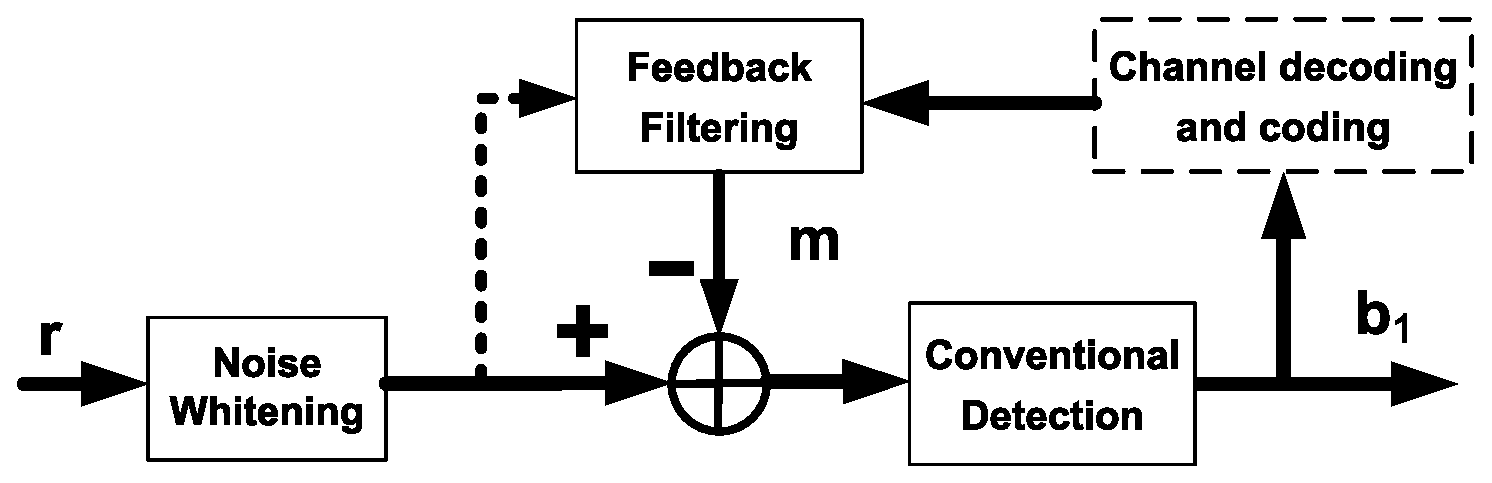
\includegraphics[width=3.2in]{Code_BDFIC.eps}
\caption{A coded blind decision feedback interference
cancellation} }\label{Coded_DFIC}
\end{figure}
\section{Performance Analysis}
\subsection{\em Comparison with Existing Blind Detectors}
\begin{figure*}[t]\label{SchemComp}\small
\center{Table 1. The comparison between the proposed framework and
other detection approaches}
\begin{center}
\begin{tabular}{lcccc}
Parameters & Conv. DF-IC & Blind MMSE & Subspace Approaches & Blind DF-IC\\
\hline \hline
\textbf{Signature of desired user(s)} & $\bf\Box$ & $\mathbf\Box$ &  $\mathbf\Box$ & $\mathbf\Box$ \\
\textbf{Signature of other users} & $\mathbf\Box$ & &  \\
\textbf{Timing of desired user(s)}  & $\mathbf\Box$ & $\mathbf\Box$ & $\mathbf\Box$ & $\mathbf\Box$ \\
\textbf{Timing of other users}  & $\mathbf\Box$ & & & \\
\textbf{Received amplitudes}  & $\mathbf\Box$ & &  &\\
\textbf{ECC decoding-integratable}& $\mathbf\Box$ &&& $\mathbf\Box$ \\
\textbf{Initialization}~{\small *} &  & $\ge L$ & $\ge L$ & $M$\\
\textbf{Latency} & $K$ & $1$ & $1$ & $1$ \\
\textbf{Complexity order} & $K$ & $1$ & $1$ & $1$ \\
\hline \hline \multicolumn{5}{l}{\tiny * For blind MMSE or
subspace approaches, they typically require much more than $L$
signals before their first detection.}
\end{tabular}
\end{center}
\end{figure*}
The comparison between the proposed framework and other major
schemes is presented in Table~1. The proposed framework only
requires $M$, where $L\ge M\ge (K-G)$, previous received signal
for signal detection and its complexity is closed to conventional
detectors while other blind approaches typically requires a lots
more than $L$ signals~\cite{Madh94,Wang98,Zhang02}.
\subsection{\em Noise Enhancement}
It is known that there is a noise enhancement issue in LS-based
decorrelating detection. With conventional decorrelating
detection, the output signal-to-noise ratio (SNR) for user $k$ is
decreased by $\left[\bR_{\bs}^{+}\right]_{kk}$. Due to the noise
item $\bN$ in $\bcS$, there is an additional noise enhancement in
the proposed LS-DFIC.

Following Girko's Law, providing $\alpha=\frac{K-G}{M}$ is fixed,
the diagonal element of
$\frac{1}{M}\left(\bB_2^{+}\bb_2\right)\left(\bB_2^{+}\bb_2\right)^{\rm
H}$ can be approximated to be $1-\alpha$ with $K$, $M$
$\rightarrow\infty$~\cite{Muller}. Therefore the covariance matrix
of $\bar\bn$ can be expressed by
\begin{equation}
\begin{array}{rcl}
\bR_{\bar\bn}&=&\frac{2M+K-G}{M}\sigma^{2}\bI
\end{array}.\label{noise_var_new}
\end{equation}
\noindent Since $\frac{2M+K-G}{M}\sigma^{2}>\sigma^{2}$, the
receiver output noise is enhanced. This noise enhancement ratio
$\beta=\frac{2M+K-G}{M}$ is illustrated in Fig. 1.
\begin{figure}\center{
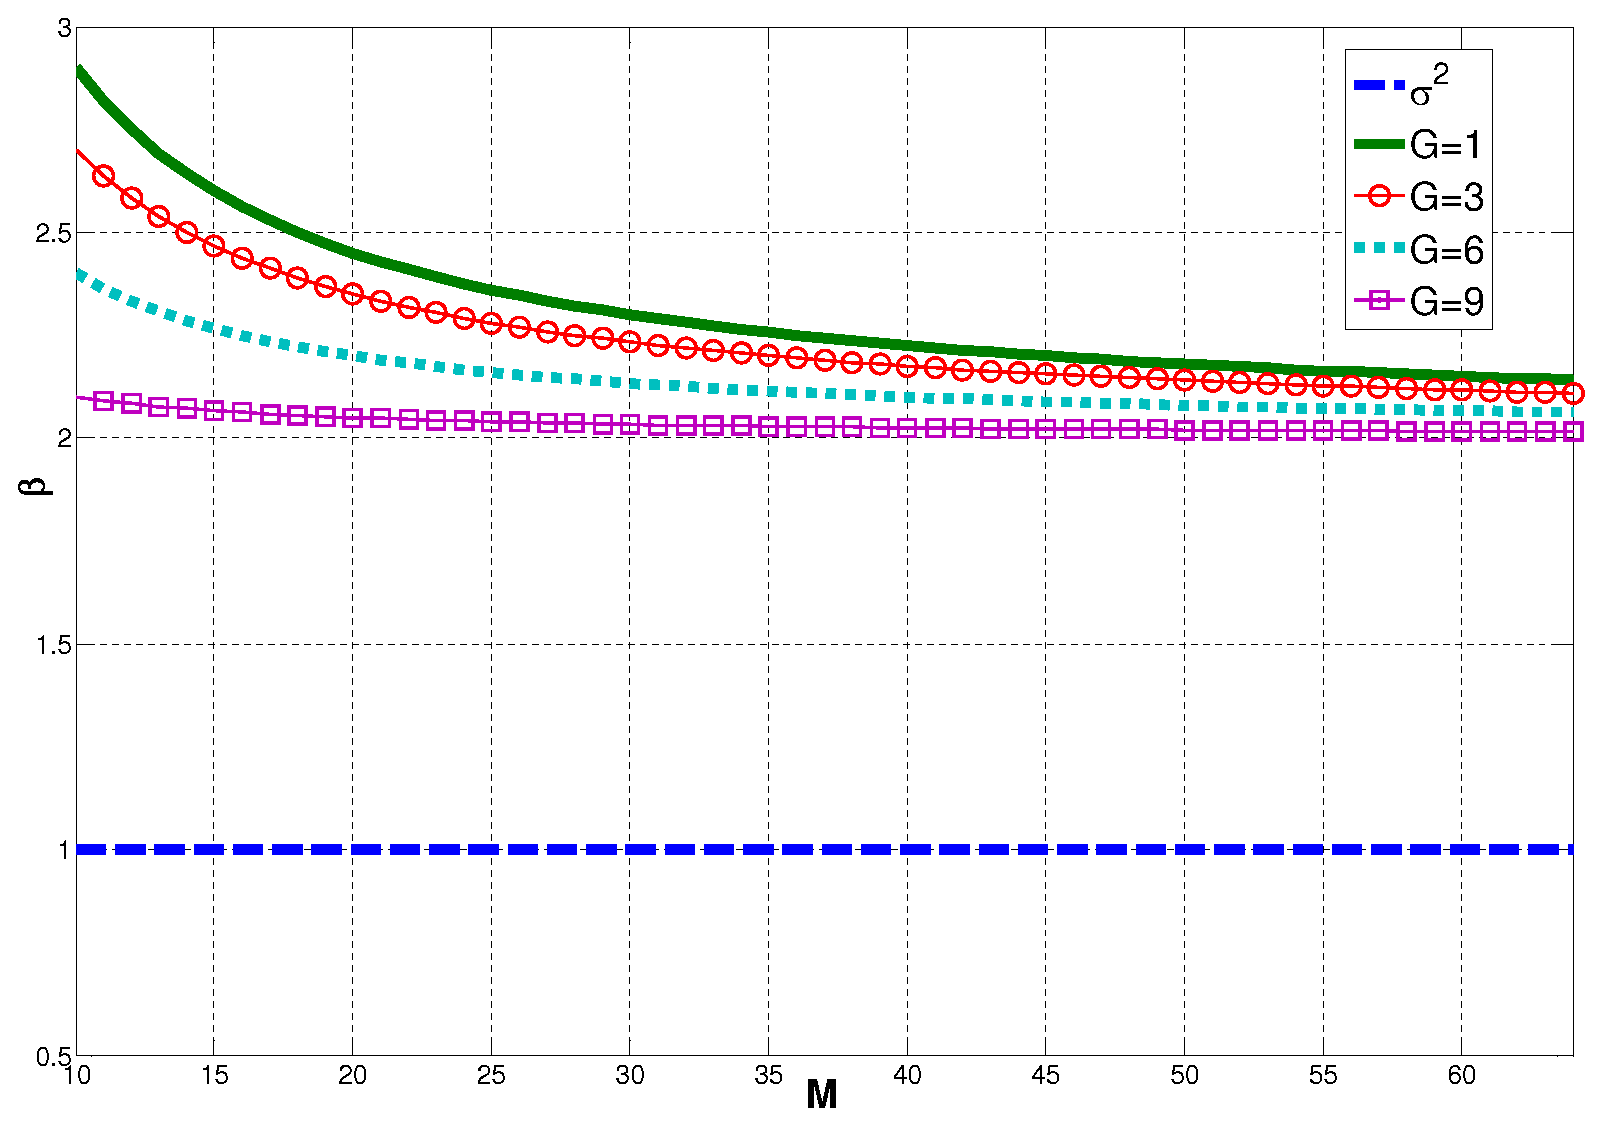
\includegraphics[width=3.0in]{noiseEnhancement2.eps}
\caption{ The noise enhancement, $K=10$ and $L=64$. }
}\label{BER_SNR}
\end{figure}
\subsection{\em AME and Near-Far Resistance}
A commonly used performance measure for a multiuser detector is
asymptotic multiuser efficiency (AME) and NFR~\cite{Verd98}. The
AME of the proposed schemes is
\begin{equation}
\begin{array}{rcl}
\bar{\eta}_k&=&{\frac{M}{2M+G-K}}\left[\bR_{\bs}^{+}\right]_{kk}^{-1}
\end{array}.
\end{equation}
\subsection{\em CRLB for $\bd_1$ and $\bbf$ Estimation}
The Cram\'{e}r-Rao Lower Bound (CRLB) is given by the inverse of
the Fisher information matrix (FIM). Providing $\bcS$ and $\bD_1$
are known beforehand, we first define the parameter vector
$\mathbf{\phi} = \left[\bar{\sigma}^{2}\ \bd_1^{\rm T}\ \bbf^{\rm
T}\right]^{\rm T}$, where $\bar{\sigma}^{2}
=(1+\frac{M}{M+G-K})\sigma^{2}$, for computing the FIM
\begin{equation}
\begin{array}{rcl}
{\bI(\mathbf{\phi})} &=& {\rm E} \left\{ \left( \frac{\partial
\ln{\cal L}}{\partial \mathbf{\phi}} \right) \left( \frac{\partial
\ln{\cal L}}{\partial \mathbf{\phi}} \right)^{\rm T} \right\}
\label{fim}
\end{array}
\end{equation}
\noindent where $\ln{\cal L}$ is the log-likelihood function given
by
\begin{equation}
\begin{array}{rcl}
\ln{\cal
L}&=&C-L\ln\bar{\sigma}^2-\frac{1}{2\bar{\sigma}^2}\parallel\mathbf{e}\parallel_2^2
\end{array},\label{logl}
\end{equation}
\noindent $C$ is a constant and
$\mathbf{e}=\br-\bS_1\bd_1+(\bcS-\bS_1\bD_1)\bbf$. Providing
$\bcS$ and $\bD_1$ are known, the closed-form CRLB expression of
$\bd_1$ is then given by
\begin{equation}
\begin{array}{l}
{\rm CRLB}\left(\bx\ \big\arrowvert\ \bcS,\
\bD_1\right)=(1+\frac{M}{M+G-K})\sigma^{2}\left(\bG^{\rm
H}\bG\right)^{\rm +}
\end{array}.\label{CRLB_f}
\end{equation}
\noindent where $\bx=\left[\matrix{\bd_1^{\rm T}&\bbf^{\rm
T}}\right]^{\rm T}$.
\section{Computer Simulations}
There are $K=10$ users with the group size $G=3$ and the spreading
sequences used in simulations are $64$-chip ($L=64$) random
sequences. In the computer simulations, the previous $M$ amplitude
estimates are averaged for the next detection without additional
amplitude filtering. From Fig. 3, it shows that the performance of
the MMSE interference cancellor is comparable to single-user
matched filter (SU-MF) and the decorrelating detector when
interfering signal power is small. When the interfering signal
power becomes larger, the SU-MF suffers from the near-far issue
and BER performance become very bad since its near-far resistance
is small. However, the MMSE interference cancellor as well as the
LS interference cancellor still works very well with strong
near-far resistance. In Fig. 4, the near-far resistance of the
proposed interference cancellors is checked with changing
interfering signal power. We can see that the both the LS-based
and MMSE-based interference cancellors have good resistance to
interferences. But compared with the conventional decorrelating
detection, these decision-feedback interference cancellors have a
higher noise floor. This is also confirmed in the previous
analysis.
\begin{figure}%\hspace{0.5in}
\center{
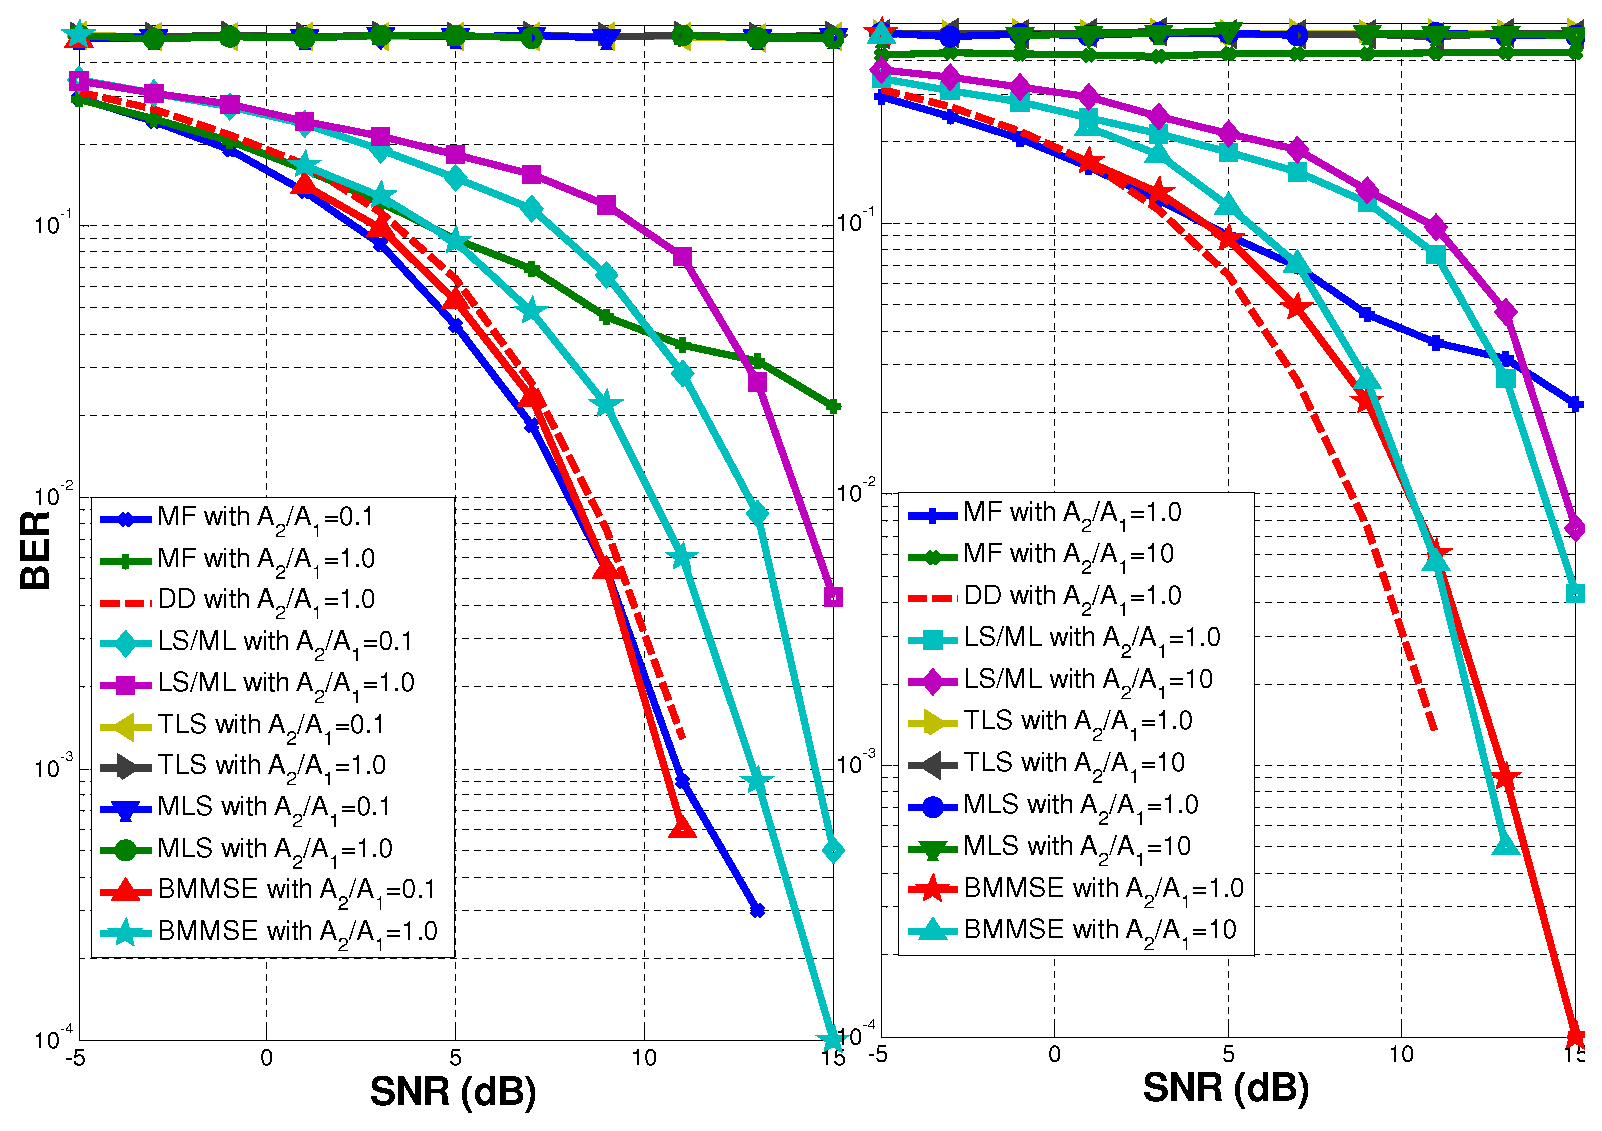
\includegraphics[width=3.0in]{BER_40_10_3_D.eps}
\caption{ The performance of the proposed blind DF-ICs against
SNR, $G=3$, $K=10$ and $M=40$. } }\label{BER_SNR}
\end{figure}
\begin{figure} \center{
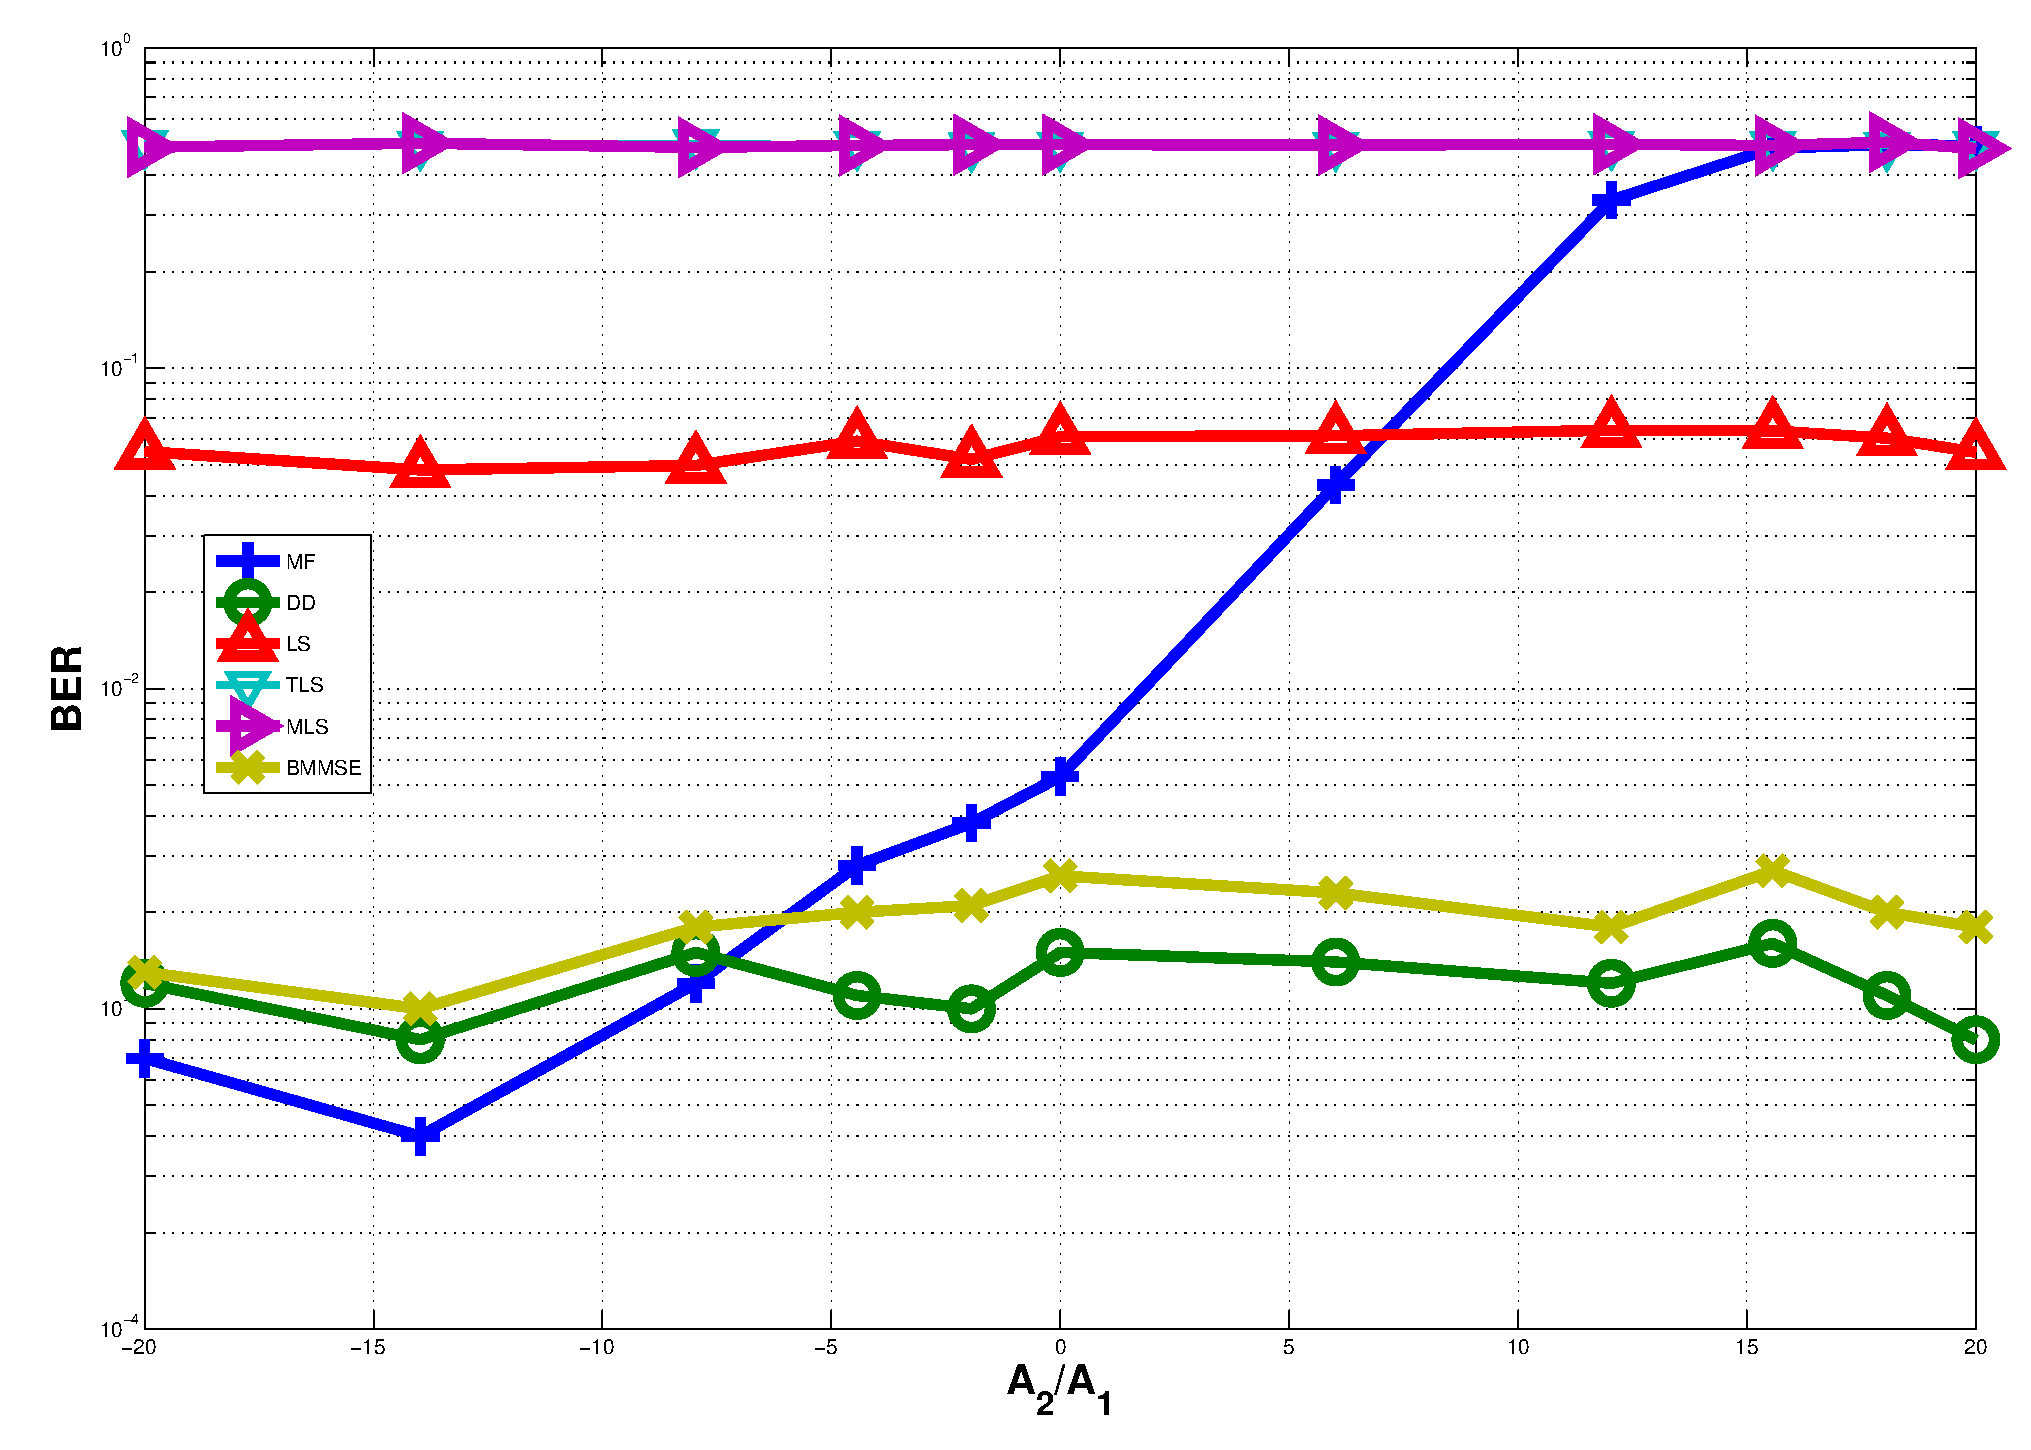
\includegraphics[width=3.2in]{NFR_10_40_2_1.eps}
\caption{ The near-far resistance performance of the proposed
DF-IC, $M=40$, $K=2$, $G=1$ and ${\rm SNR}=10{\rm dB}$.}
}\label{BER_A_SNR}
\end{figure}
\section{Conclusions}
In this paper, a blind interference cancellation framework and
several implementations of it are presented. They are simple and
direct and require a minimum amount of previous received and
detected symbols. Therefore, their implementation complexity and
detection delay can be much lower, especially when it is
implemented in adaptive and iterative fashion. Besides the
implementation considerations, we also discussed their performance
in terms of BER, AME, CRLB, etc. and compare it with other
existing multiuser receiver designs.  Some tradeoffs between
complexity and performance gain for multiuser receiver design are
revealed. Computer simulation results are provided to support our
conclusions.

\bibliographystyle{unsrt}
\bibliography{FastBDD,InterferenceCancellation}
\end{document}
